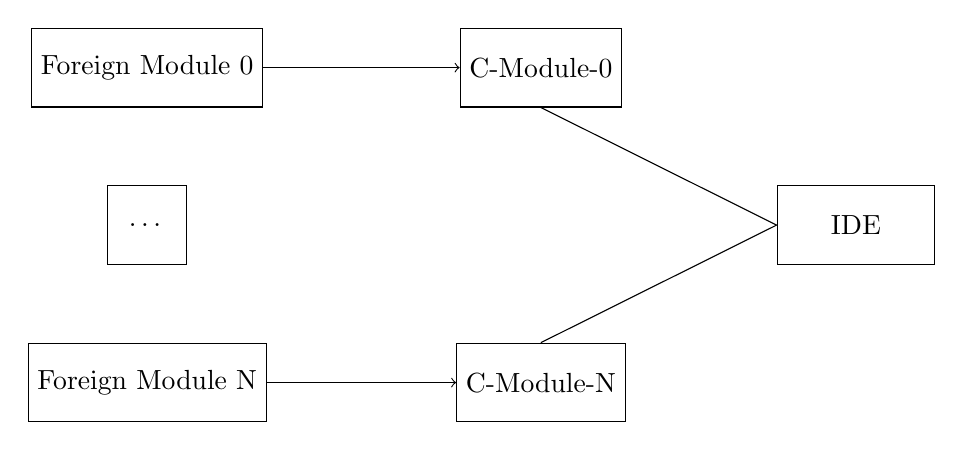
\begin{tikzpicture}
  % Nodes
  \node (p-0) [rectangle, draw, minimum height=1cm, minimum width=2cm] at (-6, 2) {Foreign Module 0};
  \node (dots) [rectangle, draw, minimum height=1cm, minimum width=1cm] at (-6, 0) {\dots};
  \node (p-n) [rectangle, draw, minimum height=1cm, minimum width=2cm] at (-6, -2) {Foreign Module N};
  \node (m-1) [rectangle, draw, minimum height=1cm, minimum width=2cm] at (-1, 2) {C-Module-0};
  \node (m-n) [rectangle, draw, minimum height=1cm, minimum width=2cm] at (-1, -2) {C-Module-N};
  \node (i) [rectangle, draw, minimum height=1cm, minimum width=2cm] at (3, 0) {IDE};
  % Arrow
  \draw (m-1.south) -- (i.west);

  \draw (m-n.north) -- (i.west);

  \draw[->] (p-0) -- (m-1);
  \draw[->] (p-n) -- (m-n);
\end{tikzpicture}
